\section{Auswertung}
\label{sec:Auswertung}

%%%%%%%%%%%%%%%%%%%%%%%%%%%%%%%%%%%%%%%%%%%%%%%%%%%%%%%%%%%%%%%%%%%%%%%%%%%%%%%%%%%%%%%%%%%%%%%%%%%%%%%%%%%%%%%%%%%%%%%%%%%%%%%%%%%

\subsection{Energiekalibrierung anhand des Spektrums von $\ce{^{152}}$Europium}

Zur Energiekalibrierung des Detektors wird das Spektrum eines $\ce{^{152}Eu}$-Strahlers aufgenommen, welches in Abbildung
\ref{fig:plot1} zu sehen ist.

\begin{figure}
  \centering
  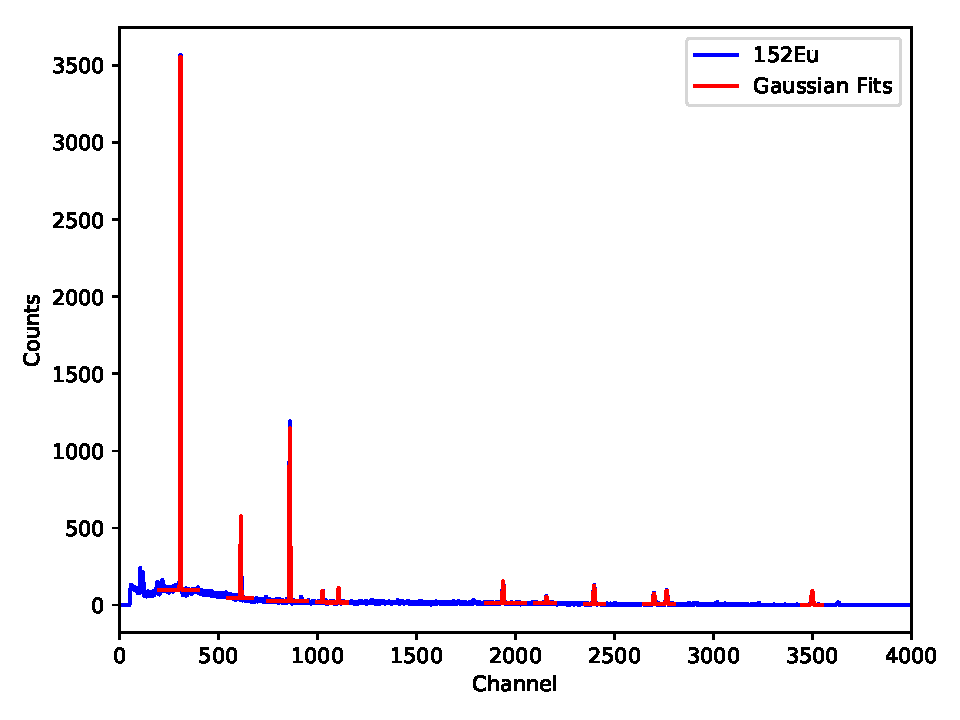
\includegraphics{content/plot1.pdf}
  \caption{Gemessenes Spektrum eines $\ce{^{152}Eu}$-Strahlers, abgeschnitten ab Kanalnummer $\num{4000}$}
  \label{fig:plot1}
\end{figure}

Dazu werden anhand der charakteristischen Peaks des Spektrums mittels linearer Regression Peakenergien $E$ und mittlere 
Kanalnummern $\mu_0$ in Beziehung gesetzt.
Die Peaks werden als Gaußverteilungen der Form 

\begin{equation}
  f(x) = a \cdot \text{exp}\left( - \frac{(x-\mu_0)^2}{b}\right) + c
\end{equation}

genähert. Dazu wird die Funktion \textit{scipy.optimize.curve\_fit} aus der Python-Bibliothek SkiPy verwendet.

Die den Peakenergien $E$ zugeordneten Näherungsparameter sind in Tabelle \ref{tab:mess1} aufgelistet.

\begin{table}
  \centering
  \caption{Gefittete Parameter der Gaußnäherungen der charakteristischen Peaks des $\ce{^{152}Eu}$-Spektrums}
  \label{tab:mess1}
  \sisetup{table-format=2.1}
  \begin{tabular}{c c c c c}
  \toprule
  $ E \;/\; \si{\kilo\eV}$ & $\mu_0$ & $a$ & $b$ & $c$ \\
  \midrule
        121,78 &  308,80 $\pm$ 0,01 & 3493,0 $\pm$ 15,0 &  3,5 $\pm$ 0,0 & 100,3 $\pm$ 1,3 \\
        244,70 &  613,80 $\pm$ 0,03 &  535,0 $\pm$  9,0 &  4,2 $\pm$ 0,2 &  45,6 $\pm$ 1,1 \\
        344,30 &  860,70 $\pm$ 0,01 & 1140,0 $\pm$  6,0 &  5,5 $\pm$ 0,1 &  24,4 $\pm$ 0,6 \\
        411,12 & 1026,51 $\pm$ 0,09 &   74,7 $\pm$  3,5 &  5,7 $\pm$ 0,6 &  18,9 $\pm$ 0,8 \\
        443,96 & 1107,93 $\pm$ 0,06 &   94,2 $\pm$  3,0 &  6,4 $\pm$ 0,5 &  16,7 $\pm$ 0,5 \\
        778,90 & 1938,62 $\pm$ 0,05 &  143,3 $\pm$  2,4 & 14,3 $\pm$ 0,5 &  11,7 $\pm$ 0,3 \\
        867,37 & 2158,39 $\pm$ 0,17 &   42,5 $\pm$  2,1 & 17,1 $\pm$ 2,0 &  10,7 $\pm$ 0,4 \\
        964,08 & 2398,18 $\pm$ 0,06 &  120,3 $\pm$  2,2 & 19,3 $\pm$ 0,8 &   6,4 $\pm$ 0,5 \\
       1085,90 & 2700,41 $\pm$ 0,14 &   67,5 $\pm$  2,2 & 30,2 $\pm$ 2,3 &   5,3 $\pm$ 0,5 \\
       1112,10 & 2765,02 $\pm$ 0,11 &   88,5 $\pm$  2,6 & 23,2 $\pm$ 1,7 &   5,6 $\pm$ 0,9 \\
       1408,00 & 3499,69 $\pm$ 0,07 &   90,7 $\pm$  1,4 & 28,9 $\pm$ 1,1 &   0,9 $\pm$ 0,3 \\
  \bottomrule
  \end{tabular}
  \end{table}

Mit den Wertepaaren der Peakenergien $E$ und der mittleren Kanalnummern $\mu$ wird eine lineare Regression der Form

\begin{equation}
  E(\mu) = m \cdot \mu_0 + d
  \label{eqn:eich}
\end{equation}
  
durchgeführt, die in Abildung \ref{fig:plot5} dargestellt ist.
Die Regressionsparameter betragen

\begin{align*}
  m &= \num{0.403 +- 0.000} \\
  d &= \num{-2.683 +- 0.051} \; .
\end{align*}

\begin{figure}
  \centering
  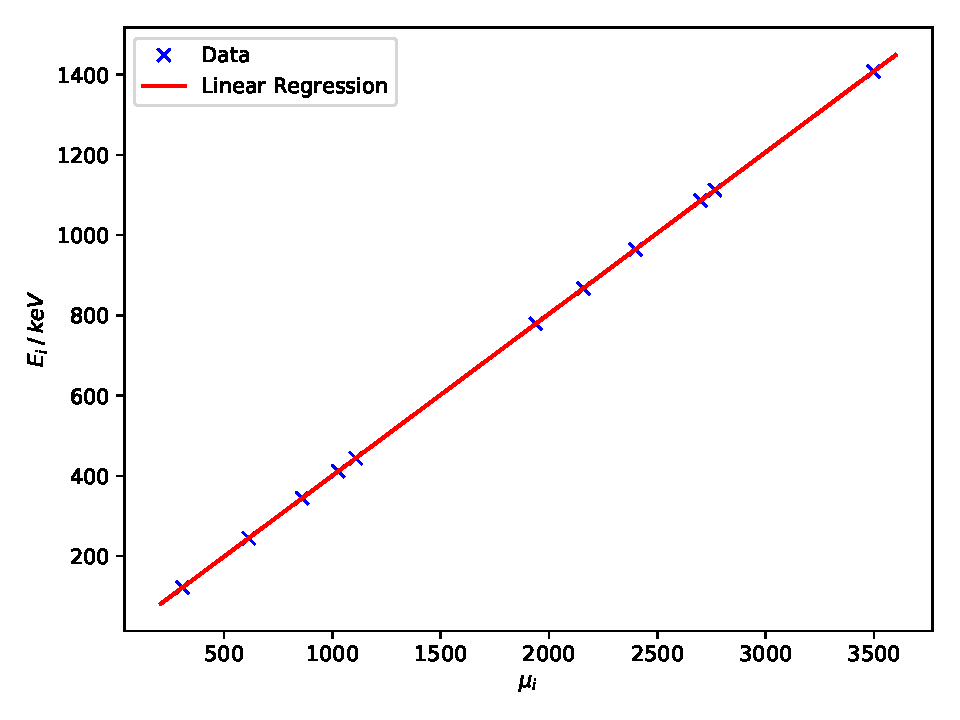
\includegraphics{content/plot5.pdf}
  \caption{Lineare Regression der Energie-Kanalnummer-Wertepaare des $\ce{^{152}Eu}$}
  \label{fig:plot5}
\end{figure}

Die statistischen Fehler der Regressionskonstanten sind mit $\SI{0.0}{\percent}$ und $\SI{1.9}{\percent}$ sehr gering.

%%%%%%%%%%%%%%%%%%%%%%%%%%%%%%%%%%%%%%%%%%%%%%%%%%%%%%%%%%%%%%%%%%%%%%%%%%%%%%%%%%%%%%%%%%%%%%%%%%%%%%%%%%%%%%%%%%%%%%%%%%%%%%%%%

\subsection{Bestimmung der Effizienz bzw. Vollenergienachweiswahrscheinlichkeit anhand des Spektrums von $\ce{^{152}}$Europium}

Die Effizienz

\begin{equation}
  Q = \frac{4 \pi Z}{\Omega A W t}
\end{equation}

wird aus dem Zählergebnis $Z$, dem Raumwinkel $\Omega$, der Aktivität $A$ des Strahlers, 
der Emmisionswahrscheinlichkeit $W$ und der Messzeit $t = \SI{4111}{\second}$ bestimmt.

Der Raumwinkel ergibt sich zu 

\begin{equation}
  \Omega = 2 \pi \left(1 - \frac{l}{\sqrt{l^2 + r^2}}\right) \approx \num{0.0538} \pi \; ,
\end{equation} 

mit dem Radius $r = \SI{2.25}{\centi\meter}$ und dem Abstand $l = \SI{9.5}{\centi\meter}$ zwischen Probe und Detektor.

Die Aktivität am Messtag wird bestimmt als

\begin{equation}
  A(t) = A_0 \cdot \text{exp} \left(- \frac{\text{ln}(2)}{t_{\sfrac{1}{2}}} \cdot t \right)  \; .
\end{equation}

Mit einer Anfangsaktivität $A_0 = \SI{4130 +- 60}{\becquerel}$ am 01.10.2000 und der Halbwertszeit
$t_{\sfrac{1}{2}} = \SI{4943 +- 5}{\day}$ ergibt sich nach einer Zeit von $t = \SI{7177}{\day}$
eine Aktivität von $A_{25.05.2020} = \SI{1510 +- 22}{\becquerel}$.
Der statistische Fehler von $A_{25.05.2020}$ ergibt sich nach 
Gaußscher Fehlerfortpflanzungaus denen von $A_0$ und $t_{\sfrac{1}{2}}$.

Zuletzt sind noch die Zählraten $Z$ der Peaks zu bestimmen. Dazu werden die gefitteten Gaußnäherungen integriert. 
Der konstante Parameter $b$ wird dabei vernachlässigt, da er das Niveau des umgebenden Spektrums angibt und somit nicht zur 
Zählrate $Z$ des Peaks beiträgt. Aus der Integration folgt dann

\begin{equation}
  Z = \int_{-\infty}^\infty \; a \cdot \text{exp}\left( - \frac{(x-\mu_0)^2}{b}\right) \; \text{d}x = a \sqrt{b\pi} \; .
\end{equation}

Der statistische Fehler der Zählrate wird aufgrund des poissonverteilten Zerfallswahrscheinlichkeit als $\sqrt{Z}$ angenommen.

In der erweiterten Tabelle \ref{tab:mess2} sind die errechneten Effizienzen $Q$, Zählraten $Z$ und 
Emmisionswahrscheinlichkeiten $W$ aufgeführt.

\begin{table}
  \centering
  \caption{Effizienzen und zu deren Berechnung notwendige Größen des $\ce{^{152}Eu}$-Strahlers}
  \label{tab:mess2}
  \sisetup{table-format=2.1}
  \begin{tabular}{c c c c c c}
  \toprule
  $E \;/\; \si{\kilo\eV}$ & $W \;\text{in}\; \si{\percent}$ & $a$ & $b$ & $Z$ & $Q$ \\
  \midrule
        121,78 & 28,6 & 3493,0 $\pm$ 15,0 &  3,5 $\pm$ 0,0 & 11582,64 $\pm$ 107,62 & 0.0048506 $\pm$  7,37 $\cdot 10^{-5}$ \\
        244,70 &  7,6 &  535,0 $\pm$  9,0 &  4,2 $\pm$ 0,2 &  1943,36 $\pm$  44,08 & 0.0030626 $\pm$  9,98 $\cdot 10^{-5}$ \\
        344,30 & 26,5 & 1140,0 $\pm$  6,0 &  5,5 $\pm$ 0,1 &  4738,72 $\pm$  68,84 & 0.0021417 $\pm$  3,85 $\cdot 10^{-5}$ \\
        411,12 &  2,2 &   74,7 $\pm$  3,5 &  5,7 $\pm$ 0,6 &   316,11 $\pm$  17,78 & 0.0017209 $\pm$ 12,38 $\cdot 10^{-5}$ \\
        443,96 &  3,1 &   94,2 $\pm$  3,0 &  6,4 $\pm$ 0,5 &   422,39 $\pm$  20,55 & 0.0016320 $\pm$  8,56 $\cdot 10^{-5}$ \\
        778,90 & 12,9 &  143,3 $\pm$  2,4 & 14,3 $\pm$ 0,5 &   960,48 $\pm$  30,99 & 0.0008918 $\pm$  2,52 $\cdot 10^{-5}$ \\
        867,37 &  4,2 &   42,5 $\pm$  2,1 & 17,1 $\pm$ 2,0 &   311,50 $\pm$  17,65 & 0.0008883 $\pm$  6,92 $\cdot 10^{-5}$ \\
        964,08 & 14,6 &  120,3 $\pm$  2,2 & 19,3 $\pm$ 0,8 &   936,74 $\pm$  30,61 & 0.0007685 $\pm$  2,40 $\cdot 10^{-5}$ \\
       1085,90 & 10,2 &   67,5 $\pm$  2,2 & 30,2 $\pm$ 2,3 &   657,48 $\pm$  25,64 & 0.0007720 $\pm$  4,03 $\cdot 10^{-5}$ \\
       1112,10 & 13,6 &   88,5 $\pm$  2,6 & 23,2 $\pm$ 1,7 &   755,55 $\pm$  27,49 & 0.0006654 $\pm$  3,27 $\cdot 10^{-5}$ \\
       1408,00 & 21,0 &   90,7 $\pm$  1,4 & 28,9 $\pm$ 1,1 &   864,23 $\pm$  29,40 & 0.0004929 $\pm$  1,41 $\cdot 10^{-5}$ \\
  \bottomrule
  \end{tabular}
  \end{table}

Um eine Potenzfunktion mit Zusammenhang zwischen Effizienz und Energie zu bestimmen,
werden die logarithmierte Effizienzen der Peaks gegen deren logarithmierten Energien aufgetragen und eine
lineare Regression der Form

\begin{equation}
  \text{ln}(Q) = n \cdot \text{ln}(\frac{E}{\SI{1}{\kilo\eV}}) + e
\end{equation}

durchgeführt, die in Abbildung \ref{fig:plot6} dargestellt ist.

\begin{figure}
  \centering
  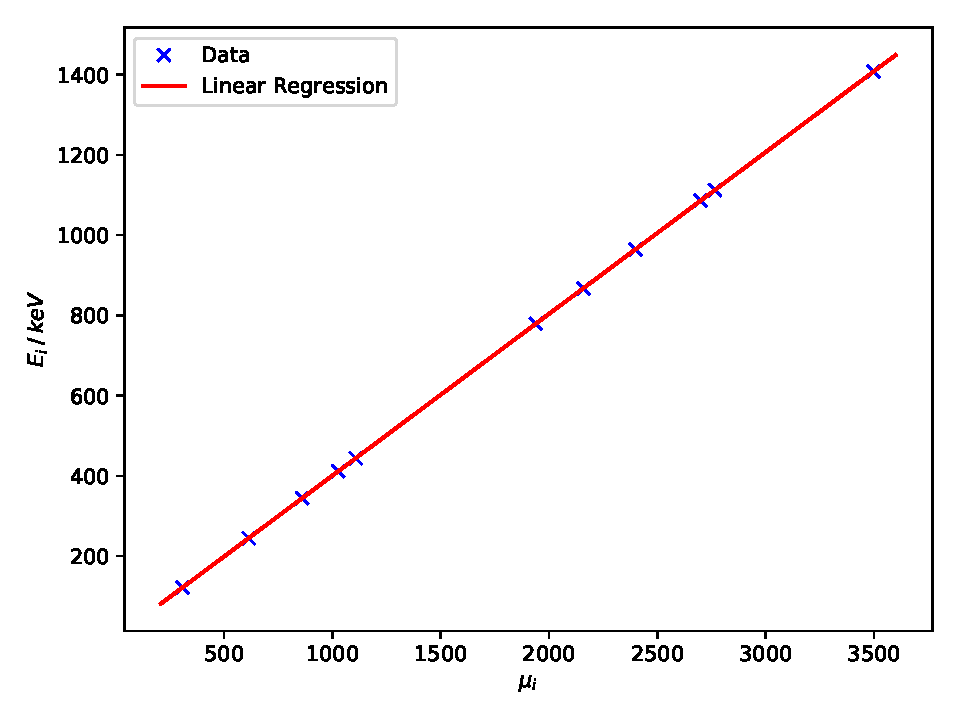
\includegraphics{content/plot6.pdf}
  \caption{Lineare Regression der logarithmierten Effizienzen abhängig von den logarithmierten Energien}
  \label{fig:plot6}
\end{figure}

Es ergeben sich die Regressionsparameter

\begin{align*}
  n &= \num{-0.934 +- 0.035} \\
  e &= \num{-0.742 +- 0.221} \; 
\end{align*}

und somit der Zusammenhang

\begin{equation}
  Q(E) = \text{e}^e \cdot \left(\frac{E}{\SI{1}{\kilo\eV}}\right)^n 
  \approx \num{0.476} \cdot \left(\frac{E}{\SI{1}{\kilo\eV}}\right)^{\num{-0.934}} \; .
\end{equation}

%%%%%%%%%%%%%%%%%%%%%%%%%%%%%%%%%%%%%%%%%%%%%%%%%%%%%%%%%%%%%%%%%%%%%%%%%%%%%%%%%%%%%%%%%%%%%%%%%%%%%%%%%%%%%%%%%%%%%%%%%%%%%%%%%%%%%%%%%%%%%

\subsection{Untersuchung des monochromatischen Gammaspektrums von $\ce{^{137}}$Caesium}

Das gemessene Spektrum von $\ce{^{137}Cs}$ ist in den Abbildungen \ref{fig:plot2} und \ref{fig:plot21} dargestellt.

\begin{figure}
  \centering
  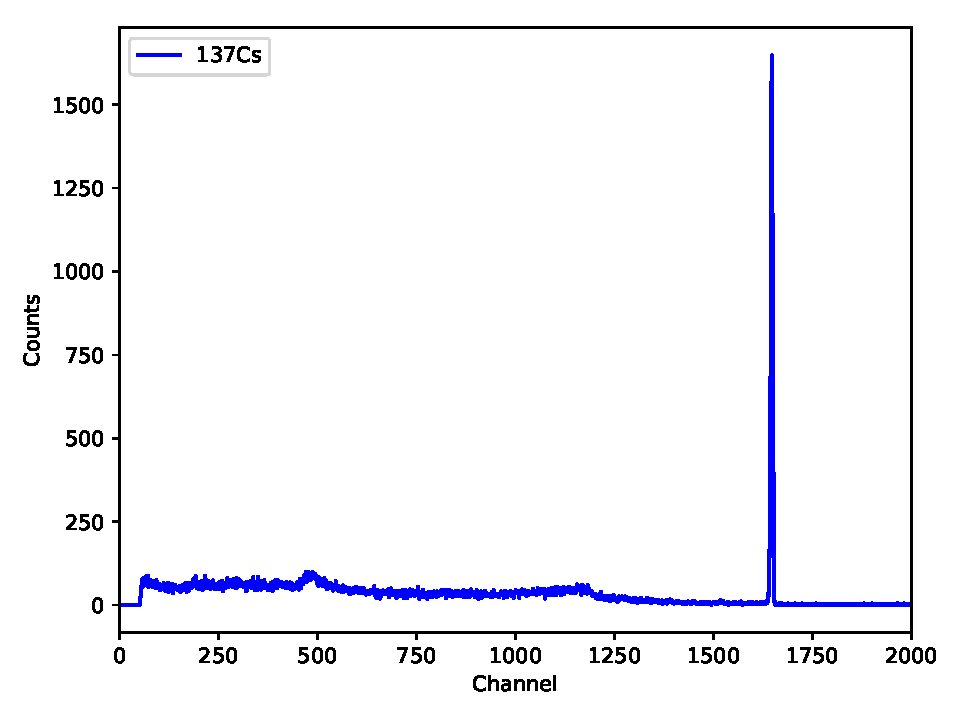
\includegraphics{content/plot2.pdf}
  \caption{Gemessenes Spektrum eines $\ce{^{137}Cs}$-Strahlers, abgeschnitten ab Kanalnummer $\num{2000}$. Hier ist der
  Photopeak bzw. Vollenergielinie gut zu erkennen.}
  \label{fig:plot2}
\end{figure}

\begin{figure}
  \centering
  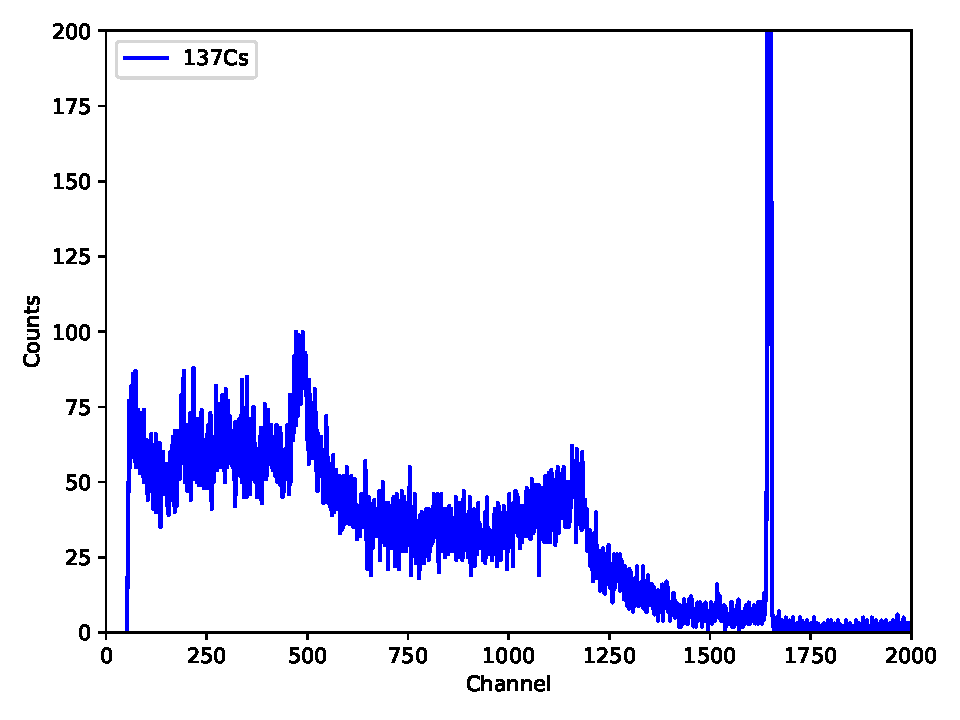
\includegraphics{content/plot21.pdf}
  \caption{Gemessenes Spektrum eines $\ce{^{137}Cs}$-Strahlers, abgeschnitten ab Kanalnummer $\num{2000}$. Zur Erkennung
    des Compton-Kontinuums, des Rückstreupeaks und der Compton-Kante wurde ein kleinerer Bereich der Ereignisanzahl gewählt.}
  \label{fig:plot21}
\end{figure}

Um die Lage des Photopeaks bzw. der Vollenergielinie zu bestimmen, wird dieser durch eine Gaußglocke genähert, die in Abbildung
\ref{fig:plot22} dargestellt ist.

\begin{figure}
  \centering
  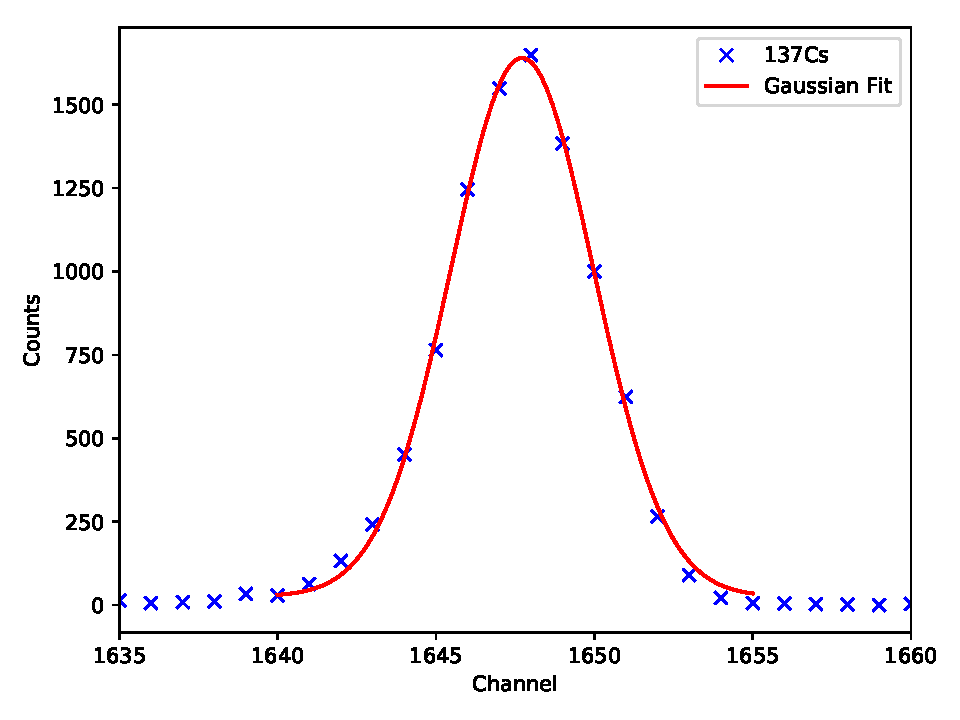
\includegraphics{content/plot22.pdf}
  \caption{Gemessener und gaußgenäherter Photopeak eines $\ce{^{137}Cs}$-Strahlers}
  \label{fig:plot22}
\end{figure}

Die Näherung erfolgt mittels der Funktion \textit{scipy.optimize.curve\_fit} aus der Python-Bibliothek SkiPy und für
das Maximum der Gaußglocke ergibt sich die Kanalnummer

\begin{equation*}
  \mu_{0,\text{Photo}} = \num{1647.72} \approx \num{1648} \; ,
\end{equation*}

die als Zentrum des Photopeaks angenommen wird.

Mit der Energieeichung \eqref{eqn:eich} lässt sich die Energie des Photopeaks als

\begin{equation*}
  E_\text{Photo} = \SI{661.35 +- 0.05}{\kilo\eV}
\end{equation*}

bestimmen.

Der Literaturwert beträgt $E_\text{Photo, Lit} = \SI{661.657}{\kilo\eV}$ [1]. Die Abweichung vom Literaturwert 
von ca. $\SI{0.3}{\kilo\eV}$ liegt über der statistischen Abweichung der Energieeichung, 
ist mit $\SI{0.046}{\percent}$ aber dennoch sehr klein.

Die maximale Ereignisanzahl des gaußgenäherten Photopeaks aus Abbildung \ref{fig:plot22} beträgt $\num{1639.91}$.
Es lassen sich die Halb- und Zehntelwertsbreiten 

\begin{align*}
  \mu_{0, \sfrac{1}{2}} &\approx \num{5.37} \\
  \mu_{0, \sfrac{1}{10}} &\approx \num{10.02}
\end{align*} 

ablesen.

Mit der Energieeichung \eqref{eqn:eich} lassen sich diese in die Energien

\begin{align*}
  \Delta E_{\sfrac{1}{2}} &\approx \SI{0.52 +- 0.05}{\kilo\eV} \\
  \Delta E_{\sfrac{1}{10}} &\approx \SI{1.36 +- 0.05}{\kilo\eV}
\end{align*}

umrechnen.

Dabei ist das Verhältnis zwischen Halb- Zehntelwertsbreiten

\begin{equation}
  \kappa = \frac{\mu_{0, \sfrac{1}{10}}}{\mu_{0, \sfrac{1}{2}}} = \frac{\Delta E_{\sfrac{1}{10}}}{\Delta E_{\sfrac{1}{2}}} = \num{1.8659}
\end{equation}

und weicht damit um nur $\SI{2.35}{\percent}$ von dem für Gaußverteilungen typischen Wert von $\kappa = \num{1.823}$ ab.

Zum Vergleich mit der gemessenen kann die Halbwertsbreite der Gaußverteilung wie folgt genähert und berechnet werden:

\begin{align}
  \Delta E_{\sfrac{1}{2}, \text{theo}} &= \sqrt{8 \cdot \text{ln}(2)} \cdot \sigma \approx \num{2.35} \cdot \sqrt{F E_\text{Photo} E_\text{Ex}} \\
  &= \num{2.35} \cdot \sqrt{\num{0.1}\cdot \SI{661.35 +- 0.05}{\kilo\eV} \cdot \SI{2.9}{\eV}} = \SI{1029.16 +- 0.04}{\eV} \; .
\end{align}

Dabei beschreibt $\sigma$ die Standartabweichung der Gaußverteilung. $E_\text{Ex}$ gibt die
Exzitonenbildungsenergie für Germanium bei einer Temperatur von $\SI{77}{\kelvin}$ an und der Fano-Faktor $F$
berücksichtigt, dass Fluktuationen in der Ladungsträger- bzw. Exzitonenerzeugung
durch Fluktuation der Photonenanregung ausgeglichen werden.

Die gemessene Halbwertsbreite $\Delta E_{\sfrac{1}{2}} \approx \SI{0.52 +- 0.05}{\kilo\eV}$ weicht um etwa
\SI{49.47}{\percent} von der theoretischen $\Delta E_{\sfrac{1}{2}, \text{theo}} = \SI{1029.16 +- 0.04}{\eV}$ ab.

Dieser Fehler kommt unter anderem durch Ablesefehler und die Näherung des Photopeaks als Gaußverteilung zustande.
Die Näherung weicht für die niedrigen Wertepaare, von denen die Zehntelwertsbreite abhängt, stärker ab, als am Rest des Peaks. \\

Die Comptonkante liegt etwa bei der Kanalnummer $\mu_{0,\text{K}} = \num{1180}$ und der Rückstreupeak etwa bei
$\mu_{0, \text{R}} = \num{490}$.

Dies entspricht den Energien

\begin{align*}
  E_\text{K} &= \SI{472.86 +- 0.05}{\kilo\eV} \\
  E_\text{R} &= \SI{194.79 +- 0.05}{\kilo\eV} \; .
\end{align*}

Berechnet werden können die Energien nach den Gleichungen \eqref{eqn:Compton} und \eqref{eqn:Kante} zu

\begin{align*}
  E_\text{K, theo} &= E_\text{Photo} \cdot \frac{2 \epsilon}{1 + 2 \epsilon} = \SI{477.05 +- 0.05}{\kilo\eV} \\
  E_\text{R, theo} &= \frac{E_\text{Photo}}{1 + 2 \epsilon} =\SI{184.299 +- 0.004}{\kilo\eV} \; .
\end{align*}

Die Abweichungen zwischen gemessenen und berechneten Energien sind mit $\SI{0.88}{\percent}$ und $\SI{5.69}{\percent}$ klein. 

Zur Bestimmung der Zählraten werden für die des Comptonkontinuums die Ereignisanzahlen linksseitig der Comptonkante
und für die des Photopeaks die innerhalb des Peaks gezählt: 

\begin{align*}
  Z_\text{Compton} &= \num{53860} \\
  Z_\text{Photo} &= \num{9506} \; .
\end{align*}

Nach Gleichung \eqref{eqn:Strahl} ergibt sich für die Absorptionswahrscheinlichkeit:

\begin{equation}
  W(D) = 1 - \text{e}^{- \mu D} \; .
\end{equation}

Der Extinktionskoeffizient lässt sich für verschiedene Energien aus Abbildung \ref{fig:Ext} ablesen.
Für eine Kristalllänge von $D = \SI{4.5}{\centi\meter}$ ergeben sich dann die in Tabelle \ref{tab:mess3}
aufgelisteten Absorptionswahrscheinlichkeiten.

\begin{table}
  \centering
  \caption{Energien, Extinktionskoeffizienten und Absorpionswahrscheinlichkeiten für den Photo- und Comtoneffekt des $\ce{^{152}Eu}$-Strahlers}
  \label{tab:mess3}
  \sisetup{table-format=2.1}
  \begin{tabular}{c c c }
  \toprule
  $ $ & $\text{Photoeffekt}$ & $\text{Comptoneffekt}$ \\
  \midrule
  $E \;/\; \si{\kilo\eV}$                 & 661,35 & 0,00 bis 472,86  \\
  $\mu \;/\; \frac{1}{\si{\centi\meter}}$ & 0,006  & 0,85 bis 0,45 \\
  $W \;/\; \si{\percent}$                 & 2,66   & 86,80 bis 97,82 \\
  \bottomrule
  \end{tabular}
\end{table}

Der Vergleich der Zählraten bzw. Linieninhalte mit den Absorptionswahrscheinlichkeiten zeigt, dass die Ereignisanzahl im Photopeak 
$5 \sfrac{1}{2}$-mal geringer und die Absorptionswahrscheinlichkeit über $30$-mal kleiner ist, als im Comptonkontinuum.
Daraus ist zu schließen, dass der Comptoneffekt Einfluss auf den Photopeak hat. Compton-gestreute Photonen können im 
Detektor noch photoelektrisch wechselwirken.

%%%%%%%%%%%%%%%%%%%%%%%%%%%%%%%%%%%%%%%%%%%%%%%%%%%%%%%%%%%%%%%%%%%%%%%%%%%%%%%%%%%%%%%%%%%%%%%%%%%%%%%%%%%%%%%%%%%%%%%%%%%%%%%%%%%

\subsection{Aktivitätsbestimmung von  $\ce{^{125}}$Stibnit oder  $\ce{^{133}}$Barium }




